\begin{question}%[codigo:EAM200401AMX; concurso:EAM; ano:2004; assunto:função do segundo grau,função quadrática, funções do segundo grau; alternativa:A]
O lucro mensal de uma fábrica é dado por \(L(x) = -2x^2 + 32x - 56\), sendo \(x\) medido em milhares de peças fabricadas e \(L\) em milhões de Reais. Quando o lucro é nulo, isto é, \(-2x^2 + 32x - 56 = 0\), a quantidade de peças produtivas é a solução positiva da equação, multiplicada por mil, então a quantidade de peças para que o lucro seja nulo é:
    \begin{tasks}
        \task 2 000 ou 14 000.
        \task 3 000 ou 16 000.
        \task 4 000 ou 12 000.
        \task 5 000 ou 16 000.
        \task 7 000 ou 18 000.
    \end{tasks}
\end{question}

\begin{question}%[codigo:EAM200402AMX; concurso:EAM; ano:2004; assunto:geometria; alternativa:E]
Na figura, os segmentos \(\overline{AB}, \overline{BC}, \overline{CD}, \overline{DE}\) são respectivamente paralelos aos segmentos \(\overline{MN}, \overline{NQ}, \overline{QO}, \overline{OP}\), o ângulo \(P\hat{O}Q = 35^\circ\) e \(A\hat{B}C = 40^\circ\). O valor do ângulo \(B\hat{C}D\) é:

% \begin{figure}[h!]
    \centering
    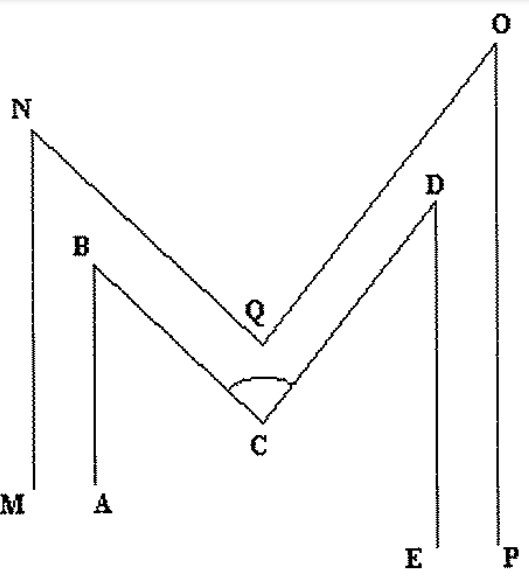
\includegraphics[width=.3\textwidth]{CONCURSO/EAM/IMAGES/2004/EAM200402IMG.png}
% \end{figure}

    \begin{tasks}
        \task \(35^\circ\).
        \task \(40^\circ\).
        \task \(50^\circ\).
        \task \(55^\circ\).
        \task \(75^\circ\).
    \end{tasks}
\end{question}

\begin{question}%[codigo:EAM200403AMX; concurso:EAM; ano:2004; assunto:regra de três; alternativa:C]
Se uma torneira enche um reservatório de água de \(5,4\) m\(^3\) a uma razão de 15 litros por minuto, quanto tempo levará para encher completamente o reservatório?
    \begin{tasks}
        \task quatro horas.
        \task cinco horas e meia.
        \task seis horas.
        \task seis horas e meia.
        \task sete horas.
    \end{tasks}
\end{question}

\begin{question}%[codigo:EAM200404AMX; concurso:EAM; ano:2004; assunto:gráfico,pizza,interpretação de gráficos; alternativa:A]
Num trabalho de pesquisa feito com \(10 000\) fumantes, divididos em 5 grupos em que a cada grupo foi aplicada uma arma contra fumo, conforme o gráfico abaixo. Sabe-se que 40\% do grupo que utilizaram a acupuntura parou de fumar. O número de pessoas que participaram dessa pesquisa e que pararam de fumar através da acupuntura é:

% \begin{figure}[h!]
    \centering
    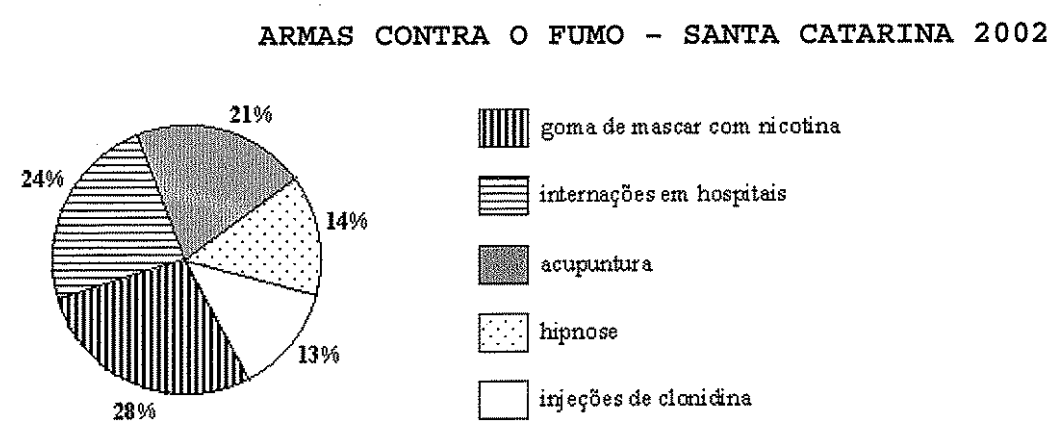
\includegraphics[width=.5\textwidth]{CONCURSO/EAM/IMAGES/2004/EAM200404IMG.png}
% \end{figure}
    \begin{tasks}
        \task \(840\).
        \task \(860\).
        \task \(1020\).
        \task \(1400\).
        \task \(1480\).
    \end{tasks}
\end{question}

\begin{question}%[codigo:EAM200405AMX; concurso:EAM; ano:2004; assunto:área, geometria; alternativa:B]
A área da figura hachurada, onde todas as medidas são em metros é: Considere \(\pi = 3,1\) e \(\sqrt{3} = 1,7\)

% \begin{figure}[h!]
    \centering
    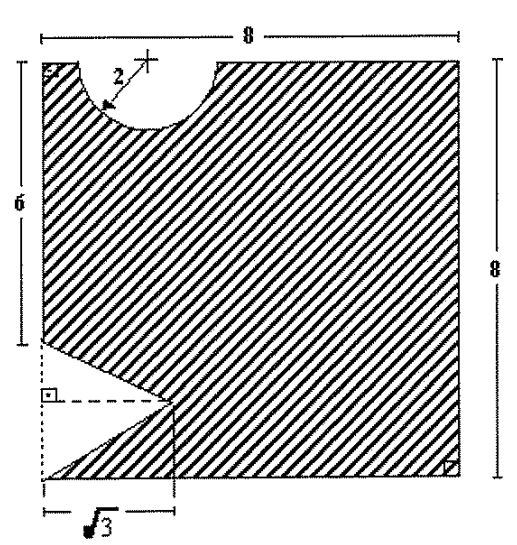
\includegraphics[width=.3\textwidth]{CONCURSO/EAM/IMAGES/2004/EAM200405IMG.png}
% \end{figure}
    \begin{tasks}
        \task \(54,1\).
        \task \(56,1\).
        \task \(58,2\).
        \task \(60,1\).
        \task \(61,3\).
    \end{tasks}
\end{question}

\begin{question}%[codigo:EAM200406AMX; concurso:EAM; ano:2004; assunto:; alternativa:B]
No painel o desenho de uma árvore de natal, na forma de um triângulo isósceles, onde a altura, e a base são números inteiros e os lados medem \(\sqrt{10}\), será revestido com um papel de parede, que custa R\$ 8,00 o metro quadrado. Qual o custo mínimo para revestir essa árvore?

% \begin{figure}[h!]
    \centering
    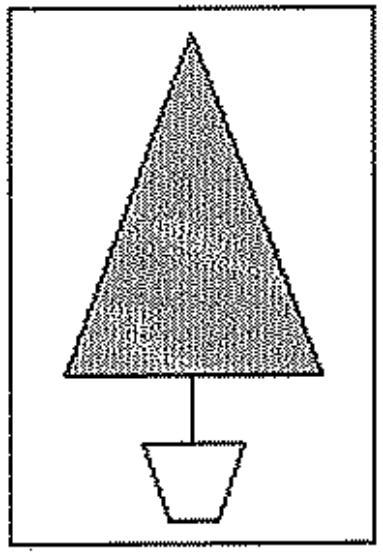
\includegraphics[width=.2\textwidth]{CONCURSO/EAM/IMAGES/2004/EAM200406IMG.png}
% \end{figure}

    \begin{tasks}
        \task R\$ 16,00.
        \task R\$ 24,00.
        \task R\$ 32,00.
        \task R\$ 40,00.
        \task R\$ 48,00.
    \end{tasks}
\end{question}

\begin{question}%[codigo:EAM200407AMX; concurso:EAM; ano:2004; assunto:; alternativa:E]
Os irmãos Antônio e Pedro, sem nenhuma economia, receberam de seu pai uma certa quantia em dólares, cada um, para fazer uma viagem. Percebendo a diferença entre essas quantias, Antônio dá a Pedro tantos dólares quanto Antônio possui. Iniciam a viagem com US\$ 1 800,00 cada um. Quantos dólares cada um recebeu de seu pai inicialmente?
    \begin{tasks}
        \task Antônio recebeu US\$ 1 000,00 e Pedro US\$ 800,00.
        \task Antônio recebeu US\$ 2 000,00 e Pedro US\$ 2 250,00.
        \task Antônio recebeu US\$ 1 350,00 e Pedro US\$ 2 600,00.
        \task Antônio recebeu US\$ 2 250,00 e Pedro US\$ 1 000,00.
        \task Antônio recebeu US\$ 2 250,00 e Pedro US\$ 1 350,00.
    \end{tasks}
\end{question}

\begin{question}%[codigo:EAM200408AMX; concurso:EAM; ano:2004; assunto:; alternativa:E]
O valor simplificado da expressão:
\[ \frac{1,363636 \ldots \times 2 \frac{1}{5} - (0,5)^2}{(\sqrt{2})^{-4}}\] é:
    \begin{tasks}
        \task \(\frac{9}{5}\).
        \task \(\frac{31}{5}\).
        \task \(7\).
        \task \(9\).
        \task \(11\).
    \end{tasks}
\end{question}

\begin{question}%[codigo:EAM200409AMX; concurso:EAM; ano:2004; assunto:; alternativa:C]
Para monitorar duas avenidas, devem ser instaladas câmeras, posicionadas em pontos a partir da posição \(1\) até a posição \(n\) nas avenidas \(A\) e \(B\). Sendo \(u\) a maior e constante distância entre as câmeras, o total de câmeras a serem instaladas nas avenidas é:

% \begin{figure}[h!]
    \centering
    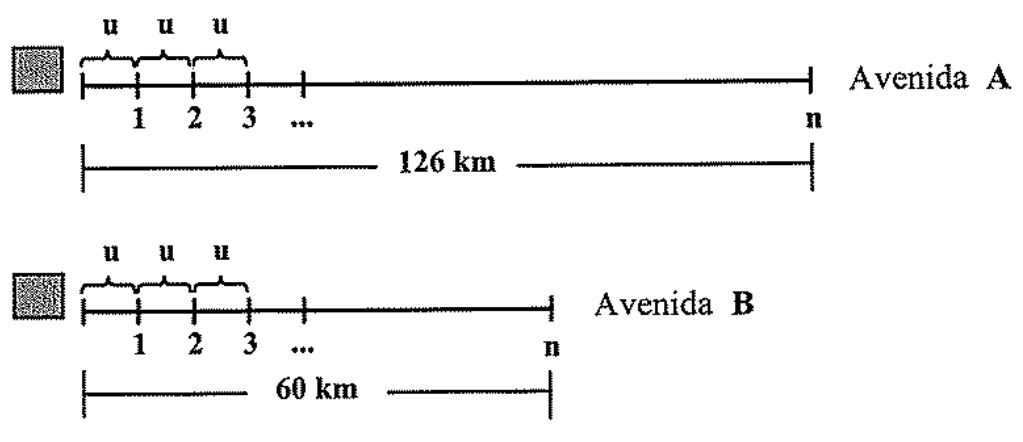
\includegraphics[width=.3\textwidth]{CONCURSO/EAM/IMAGES/2004/EAM200409IMG.png}
% \end{figure}
    \begin{tasks}
        \task \(28\).
        \task \(30\).
        \task \(31\).
        \task \(36\).
        \task \(37\).
    \end{tasks}
\end{question}

\begin{question}%[codigo:EAM200410AMX; concurso:EAM; ano:2004; assunto:; alternativa:B]
Para sustentação de letreiro é feito um suporte de ferro na forma de um triângulo retângulo \(ABC\). Calcule o comprimento de barra de ferro representada pelo segmento \(\overline{AD}\), sabendo que é bissetriz do ângulo \(B\hat{A}C\).

% \begin{figure}[h!]
    \centering
    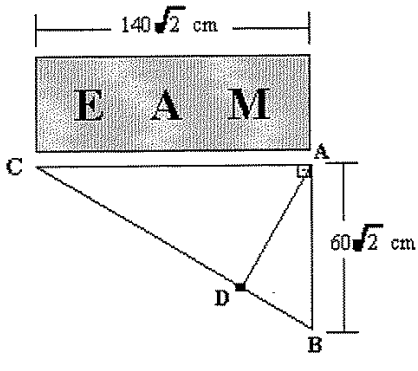
\includegraphics[width=.3\textwidth]{CONCURSO/EAM/IMAGES/2004/EAM200410IMG.png}
% \end{figure}
    \begin{tasks}
        \task \(0,56\)m.
        \task \(0,84\)m.
        \task \(0,92\)m.
        \task \(1\)m.
        \task \(1,2\)m.
    \end{tasks}
\end{question}

\begin{question}%[codigo:EAM200411AMX; concurso:EAM; ano:2004; assunto:; alternativa:A]
Em uma viagem foram colocador dois tipos de revistas para que os tripulantes de um fragata desfrutassem de uma boa leitura. Ao final da viagem foi feita uma pesquisa com todos os tripulantes para saber das preferências com relação às revistas "saúde à bordo" ou "vida marinha", verificou-se que:

\begin{itemize}
    \item 20 tripulantes leram "saúde à bordo"
    \item 30 tripulantes leram "vida marinha"
    \item 8 tripulantes leram as duas revistas
    \item 14 tripulantes não leram nenhuma dessas revistas
\end{itemize}
Qual o número de tripulantes da fragata nesta viagem?
    \begin{tasks}
        \task \(56\).
        \task \(58\).
        \task \(64\).
        \task \(68\).
        \task \(72\).
    \end{tasks}
\end{question}

\begin{question}%[codigo:EAM200412AMX; concurso:EAM; ano:2004; assunto:; alternativa:E]
Um marinheiro ao viajar comprou US\$ 1 000,00 a uma taxa de 2,9 Reais por Dólar. Não havendo usado este dinheiro na viagem, ele vendeu, na sua volta a uma taxa de 2,7 Reais por Dólar. Então:
    \begin{tasks}
        \task O marinheiro lucrou R\$ 180,00.
        \task O marinheiro lucrou R\$ 190,00.
        \task O marinheiro lucrou R\$ 200,00.
        \task O marinheiro perdeu R\$ 100,00.
        \task O marinheiro perdeu R\$ 200,00.
    \end{tasks}
\end{question}

\begin{question}%[codigo:EAM200413AMX; concurso:EAM; ano:2004; assunto:; alternativa:D]
Numa competição de arremesso de dardo, o vencedor conseguiu 82m. O segundo colocado 78m. De quanto foi o lançamento do terceiro colocado, sabendo-se que a diferença entre seu lançamento e o lançamento do segundo colocado foi a terça parte da diferença entre o seu lançamento e o do primeiro?
    \begin{tasks}
        \task \(72\)m.
        \task \(74\)m.
        \task \(75\)m.
        \task \(76\)m.
        \task \(77\)m.
    \end{tasks}
\end{question}

\begin{question}%[codigo:EAM200414AMX; concurso:EAM; ano:2004; assunto:; alternativa:D]
A somar das raízes reais da equação:
\[\sqrt{2} x^2 - (2\sqrt{2} + 2)x + 4 = 0\]
    \begin{tasks}
        \task \(0\).
        \task \(2 - \sqrt{2}\).
        \task \(\sqrt{2}\).
        \task \(2 + \sqrt{2}\).
        \task \(4\sqrt{2}\).
    \end{tasks}
\end{question}

\begin{question}%[codigo:EAM200415AMX; concurso:EAM; ano:2004; assunto:; alternativa:C]
No numeral \(213a46\), a letra \(a\) representa um algarismo. Se o número correspondente é divisível por 3, a soma dos algarismos que podem substituir a letra \(a\) é:
    \begin{tasks}
        \task \(10\).
        \task \(12\).
        \task \(15\).
        \task \(16\).
        \task \(17\).
    \end{tasks}
\end{question}
